\documentclass[10pt,a4j,dvipdfmx]{jarticle}
%---------------------------------------------------
\usepackage{hyperref}
\usepackage{pxjahyper}
\usepackage{bm}
\usepackage{graphicx}
\usepackage{amssymb,amsmath,mathtools}
\usepackage{ascmac}
\usepackage{float}
\usepackage{setspace}
\usepackage[dvips,usenames]{color}
\usepackage{colortbl}
\usepackage{algorithm}
\usepackage{algorithmic}
\usepackage{setspace}
\usepackage{subfigure}
\usepackage[deluxe,bold]{otf}
\usepackage[haranoaji]{pxchfon}
\usepackage{redeffont}
\usepackage{listings,jvlisting} %日本語のコメントアウトをする場合jvlisting(もしくはjlisting)が必要
\usepackage{booktabs}
%---------------------------------------------------
\definecolor{bl}{rgb}{0.94,0.97,1}
\definecolor{gr}{rgb}{0.5,0.5,0.5}
% \makeatletter
% \def\section{\newpage\@startsection {section}{1}{\z@}{2.3ex plus -1ex minus -.2ex}{2.3 ex plus .2ex}{\Large\bf}}
% \makeatother
%---------------------------------------------------
\setlength{\textwidth}{160truemm}
\setlength{\textheight}{240truemm}
\setlength{\topmargin}{-14.5truemm}
\setlength{\oddsidemargin}{-0.5truemm}
\setlength{\headheight}{0truemm}
\setlength{\parindent}{1zw}
\setlength{\abovedisplayskip}{-2pt} % 数式上部のマージン
\setlength{\belowdisplayskip}{0pt} % 数式下部のマージン
%---------------------------------------------------
\setstretch{1.2}
%---------------------------------------------------
\renewcommand{\subfigtopskip}{5pt}	% 図の上の隙間。上図の副題と下図の間。
\renewcommand{\subfigbottomskip}{0pt} % 図の下の隙間。副題と本題の間。
\renewcommand{\subfigcapskip}{-6pt}	% 図と副題の間
\renewcommand{\subcapsize}{\scriptsize} % 副題の文字の大きさ
\newcommand{\mysection}[1]{\newpage\vspace{-20pt}\section{#1}}
\newcommand{\mysubsection}[1]{\vspace{-20pt}\subsection{#1}}
\newcommand{\mysubsubsection}[1]{\vspace{-10pt}\subsubsection{#1}}
%---------------------------------------------------
% ヘッダーとフッターの設定
\usepackage{fancyhdr}
\rhead{\leftmark}
\chead{}
\lhead{\rightmark}
\cfoot{\thepage}

\rfoot{}
\begin{document}
%---------------------------------------------------
\setlength{\abovedisplayskip}{1.5pt} 
\setlength{\belowdisplayskip}{0pt}
%---------------------------------------------------
%ここからソースコードの表示に関する設定
\lstset{
  basicstyle={\ttfamily},
  identifierstyle={\small},
  commentstyle={\smallitshape},
  keywordstyle={\small\bfseries},
  ndkeywordstyle={\small},
  stringstyle={\small\ttfamily},
  frame={tb},
  breaklines=true,
  columns=[l]{fullflexible},
  numbers=left,
  xrightmargin=0zw,
  xleftmargin=3zw,
  numberstyle={\scriptsize},
  stepnumber=1,
  numbersep=1zw,
  lineskip=-0.5ex
}
%ここまでソースコードの表示に関する設定
%---------------------------------------------------
\pagenumbering{arabic}
\pagestyle{fancy}
\setlength{\headheight}{5truemm}

\mysection{演習19}
\subsection{実行プログラム}
実行プログラムをソースコード\ref{s19}に示す。
パラメータ値は、\textgt{RADIUS}を変化させると、
回転量が変化し、ロボットの回転と進行距離の両方が代わるため、
DISTANCEの値のみを変更した。\textgt{DISTANCE}の実測値を計測し、
DISTANCEの値を上下に変化させて、34.0から34.05に変更した。
360度回転は、指示値通りに動くが、直進の際の始動にモータの左右差が
あったため、それを考慮した上で34.05の値とした。

\begin{lstlisting}[caption=演習19のプログラム,label=s19]
#include <stdio.h>
#include <math.h>
#include <process.h>
#include <dos.h>
#include "v25.h"
#include "ms.h"

#define D2R         (M_PI/180)
#define R2D         (180/M_PI)
#define RADIUS	15.0
#define DISTANCE    34.05
#define REDUCTION   19.225
#define CPR         400
#define MMPS        (60*REDUCTION/(2.0*M_PI*RADIUS))
#define DPC         (2.0*M_PI*RADIUS/((float)CPR*REDUCTION))
#define APC         (DPC/(2*DISTANCE))
#define DMAX        1000
#define THRESH_D    10
#define THRESH_Q    5*D2R
#define THRESH_V    50

#define ABS(x)      (x<0?-(x):(x))

void estimate(double *px,double *py,double *pq,long *pt);
void translate(double d,double vmax,double gain);
void rotate(double qd,double wmax,double gain);

int k=0;
int xi[DMAX],yi[DMAX],qi[DMAX];
long ti[DMAX];

int main(void)
{
    double x,y,q;
    int i;
    int kp=8,ki_inv=8;
    int vmax = 100;
    int wmax = 100/DISTANCE;
    int nl,nr;
    long t,nt;
    FILE *fp;

    ms_init();
    ms_motor_on();
    ms_set_gain(kp,ki_inv);

    estimate(&x,&y,&q,&t);
    rotate(360*D2R,wmax,5);
    translate(1000,vmax,5);

    ms_set_v(0,0);
    do{
        estimate(&x,&y,&q,&t);
        ms_read_v(&nl,&nr,&nt);
    }while(nl != 0 || nr != 0);

    ms_motor_off();

    if((fp=fopen("data.dat","wt"))==NULL)
    {
        printf("Can't open file...\n");
    }

    for(i=0;i<k;i++)
    {
        fprintf(fp,"%5d %5d %5d %5ld\n",xi[i],yi[i],qi[i],ti[i]);
    }
    fclose(fp);
    return 0;
}

void estimate(double *px,double *py,double *pq,long *pt)
{
    static long cl0=0,cr0=0;
    static double x=0.0,y=0.0,q=0.0;
    long cl,cr,ct;
    int dl,dr;
    double ds;

    ms_read_c(&cl,&cr,&ct);
    dl=cl-cl0;
    dr=cr-cr0;
    cl0=cl;
    cr0=cr;
    ds=DPC/2*(dr+dl);
    x += ds*cos(q);
    y += ds*sin(q);
    q += APC*(dr-dl);

    *px=x;
    *py=y;
    *pq=q;
    *pt=ct;
    if (k<DMAX)
    {
        xi[k]=10*x;
        yi[k]=10*y;
        qi[k]=1000*q;
        ti[k]=ct;
        k++;
    }    

}

void translate(double d,double vmax,double gain)
{
    double x0,y0,q0,x,y,q;
    long t0,t,nt;
    double cosq0,sinq0,dd,vc;
    int nc,nl,nr;

    estimate(&x0,&y0,&q0,&t0);
    cosq0=cos(q0);
    sinq0=sin(q0);
    x=x0;
    y=y0;
    q=q0;
    t=t0;

    do
    {
        dd=cosq0*(x-x0)+sinq0*(y-y0);
        vc=gain*(d-dd);
        if (ABS(vc)>vmax)
        {
            vc=(vc<0.0)?-vmax:vmax;
        }
        nc=vc*MMPS;
        ms_set_v(nc,nc);
        estimate(&x,&y,&q,&t);
        ms_read_v(&nl,&nr,&nt);
    } while (ABS(d-dd)>THRESH_D||ABS(nl)>THRESH_V||ABS(nr)>THRESH_V);
}

void rotate(double qd,double wmax,double gain)
{
  double x0,y0,q0,x,y,q;
  long t0,t,nt;
  double qq,wc,v,dw;
  int nl,nr;

  estimate(&x0,&y0,&q0,&t0);
  x=x0;
  y=y0;
  q=q0;
  t=t0;

  do{
  qq=q-q0;
  wc=gain*(qd-qq);
  if(ABS(wc)>wmax)
  {
    wc=(wc<0.0) ? -wmax:wmax;
  }
  dw=DISTANCE*wc;
  nl=-MMPS*dw;
  nr=MMPS*dw;
  ms_set_v(nl,nr);
  estimate(&x,&y,&q,&t);
  ms_read_v(&nl,&nr,&nt);
  }while (ABS(qd-qq)>THRESH_Q||ABS(nl)>THRESH_V||ABS(nr)>THRESH_V);
}
\end{lstlisting}

\mysubsection{実行結果}
ロボットが、その場で360度回転して1000[mm]直進する。
回転角度を360度より浅くして、直進動作時に左右のモータの始動差を吸収して、
360度方向に直進する。

\mysection{演習20}
\subsection{実行プログラム}
実行プログラムをソースコード\ref{s20}に示す。
ロボットの初期位置を$(x_s, y_s, \theta_s) = (0, 0, 0)$としている。

\begin{lstlisting}[caption=演習20のプログラム,label=s20]
#include <stdio.h>
#include <math.h>
#include <process.h>
#include <dos.h>
#include "v25.h"
#include "ms.h"

#define D2R         (M_PI/180)
#define R2D         (180/M_PI)
#define RADIUS	15.0
#define DISTANCE    34.05
#define REDUCTION   19.225
#define CPR         400
#define MMPS        (60*REDUCTION/(2.0*M_PI*RADIUS))
#define DPC         (2.0*M_PI*RADIUS/((float)CPR*REDUCTION))
#define APC         (DPC/(2*DISTANCE))
#define DMAX        1000
#define THRESH_D    10
#define THRESH_Q    5*D2R
#define THRESH_V    50

#define ABS(x)      (x<0?-(x):(x))

void estimate(double *px,double *py,double *pq,long *pt);
void translate(double d,double vmax,double gain);
void rotate(double qd,double wmax,double gain);

int k=0;
int xi[DMAX],yi[DMAX],qi[DMAX];
long ti[DMAX];

int main(void)
{
    double x,y,q;
    double x_d=0,x_s=0,y_d=0,y_s=0,th_s=0,th_d=0,th_1=0,th_2=0,a_0=0;
    int i;
    int kp=8,ki_inv=8;
    int vmax = 100;
    int wmax = 100/DISTANCE;
    int nl,nr;
    long t,nt;
    FILE *fp;




    while(1){
    ms_init();
        ms_motor_on();
        ms_set_gain(kp,ki_inv);
    printf("x_d y_d th_d\n");
    scanf("%lf %lf %lf",&x_d,&y_d,&th_d);
        estimate(&x,&y,&q,&t);
    th_1=atan2(y_d-y_s,x_d-x_s)-th_s;
        rotate(th_1,wmax,5);
    a_0=sqrt((x_d-x_s)*(x_d-x_s)+(y_d-y_s)*(y_d-y_s));
        translate(a_0,vmax,5);
    th_2=th_d*D2R-th_1-th_s;
    rotate(th_2,wmax,5);
    printf("aaa\n");
    x_s=x_d;
    y_s=y_d;
    th_s=th_d;

        ms_set_v(0,0);
        do{
        estimate(&x,&y,&q,&t);
        ms_read_v(&nl,&nr,&nt);
        }while(nl != 0 || nr != 0);

    ms_motor_off();
    }
    return 0;
}

void estimate(double *px,double *py,double *pq,long *pt)
{
    static long cl0=0,cr0=0;
    static double x=0.0,y=0.0,q=0.0;
    long cl,cr,ct;
    int dl,dr;
    double ds;

    ms_read_c(&cl,&cr,&ct);
    dl=cl-cl0;
    dr=cr-cr0;
    cl0=cl;
    cr0=cr;
    ds=DPC/2*(dr+dl);
    x += ds*cos(q);
    y += ds*sin(q);
    q += APC*(dr-dl);

    *px=x;
    *py=y;
    *pq=q;
    *pt=ct;
    if (k<DMAX)
    {
        xi[k]=10*x;
        yi[k]=10*y;
        qi[k]=1000*q;
        ti[k]=ct;
        k++;
    }    

}

void translate(double d,double vmax,double gain)
{
    double x0,y0,q0,x,y,q;
    long t0,t,nt;
    double cosq0,sinq0,dd,vc;
    int nc,nl,nr;

    estimate(&x0,&y0,&q0,&t0);
    cosq0=cos(q0);
    sinq0=sin(q0);
    x=x0;
    y=y0;
    q=q0;
    t=t0;

    do
    {
        dd=cosq0*(x-x0)+sinq0*(y-y0);
        vc=gain*(d-dd);
        if (ABS(vc)>vmax)
        {
            vc=(vc<0.0)?-vmax:vmax;
        }
        nc=vc*MMPS;
        ms_set_v(nc,nc);
        estimate(&x,&y,&q,&t);
        ms_read_v(&nl,&nr,&nt);
    } while (ABS(d-dd)>THRESH_D||ABS(nl)>THRESH_V||ABS(nr)>THRESH_V);
}

void rotate(double qd,double wmax,double gain)
{
    double x0,y0,q0,x,y,q;
    long t0,t,nt;
    double qq,wc,v,dw;
    int nl,nr;

    estimate(&x0,&y0,&q0,&t0);
    x=x0;
    y=y0;
    q=q0;
    t=t0;

    do{
    qq=q-q0;
    wc=gain*(qd-qq);
    if(ABS(wc)>wmax)
    {
        wc=(wc<0.0) ? -wmax:wmax;
    }
    dw=DISTANCE*wc;
    nl=-MMPS*dw;
    nr=MMPS*dw;
    ms_set_v(nl,nr);
    estimate(&x,&y,&q,&t);
    ms_read_v(&nl,&nr,&nt);
    printf("%lf %lf %lf\n", ABS(qd-qq), ABS(nl), ABS(nr));
    }while (ABS(qd-qq)>THRESH_Q||ABS(nl)>THRESH_V||ABS(nr)>THRESH_V);
}
\end{lstlisting}

\mysubsection{実行結果}
目標位置$(x_d, y_d, \theta_d)$を入力すると、
目標方向を向き、目標の座標$(x_d, y_d)$の方向に直進し、
到着すると$\theta_d$方向に向きを変える。
目標位置・姿勢の状態をとると、初期値を現在値に更新し、
再び目標位置の入力待機を行う。その後、目標位置の入力と移動の処理を繰り返して行うことができる。
その際、目標位置の入力前にモータの電圧をオンと初期化、出力後にモータの電圧をオフ
を毎ループごとに繰り返し行う。

\mysection{演習21}
\subsection{実行プログラム}
実行プログラムをソースコード\ref{s21}に示す。

\begin{lstlisting}[caption=演習21のプログラム,label=s21]
#include <stdio.h>
#include <math.h>
#include <process.h>
#include <dos.h>
#include "v25.h"
#include "ms.h"

#define D2R         (M_PI/180)
#define R2D         (180/M_PI)
#define RADIUS	15.0
#define DISTANCE    34.05
#define REDUCTION   19.225
#define CPR         400
#define MMPS        (60*REDUCTION/(2.0*M_PI*RADIUS))
#define DPC         (2.0*M_PI*RADIUS/((float)CPR*REDUCTION))
#define APC         (DPC/(2*DISTANCE))
#define DMAX        1000
#define THRESH_D    10
#define THRESH_Q    5*D2R
#define THRESH_V    1

#define GOALX       1200
#define GOALY       1000
#define GOALQ       0
#define VMAX        150
#define WMAX        (VMAX/(3*DISTANCE))
#define REVERSE     200

#define ABS(x)      (x<0?-(x):(x))

void estimate(double *px,double *py,double *pq,long *pt);
void translate(double d,double vmax,double gain);
int translate2(double d,double vmax,double gain);
void rotate(double qd,double wmax,double gain);
double seikika(double angle);
void avoid(int j);

int k=0;
int xi[DMAX],yi[DMAX],qi[DMAX];
long ti[DMAX];

int main(void)
{
    double x,y,q,q1,q2,dl,dq;
    int i,j;
    int kp=8,ki_inv=8;
    int nl,nr;
    long t,nt;
    FILE *fp;

    ms_init();
    ms_set_gain(kp,ki_inv);
    ms_motor_on();
    ms_wait(1000);

    while (1)
    {
        estimate(&x,&y,&q,&t);

        dl=sqrt((GOALX-x)*(GOALX-x)+(GOALY-y)*(GOALY-y));
        if(dl<THRESH_D) break;

        dq=atan2(GOALY-y,GOALX-x)-q;
        dq=seikika(dq);
        rotate(dq,WMAX,5);

        j=translate2(dl,VMAX,5);

        avoid(j);
    }

    while (1)
    {
        estimate(&x,&y,&q,&t);

        dq=seikika(GOALQ-q);
        if (ABS(dq)<THRESH_Q)   break;

        rotate(dq,WMAX,5);
    }

      ms_motor_off();

    if((fp=fopen("data.dat","wt"))==NULL)
    {
        printf("Can't open file...\n");
        exit(1);
    }

    for(i=0;i<k;i++)
    {
        fprintf(fp,"%5d %5d %5d %5ld\n",xi[i],yi[i],qi[i],ti[i]);
    }
    fclose(fp);
    return 0;
}

void estimate(double *px,double *py,double *pq,long *pt)
{
    static long cl0=0,cr0=0;
    static double x=0.0,y=0.0,q=0.0;
    long cl,cr,ct;
    int dl,dr;
    double ds;

    ms_read_c(&cl,&cr,&ct);
    dl=cl-cl0;
    dr=cr-cr0;
    cl0=cl;
    cr0=cr;
    ds=DPC/2*(dr+dl);
    x += ds*cos(q);
    y += ds*sin(q);
    q += APC*(dr-dl);

    *px=x;
    *py=y;
    *pq=q;
    *pt=ct;
    if (k<DMAX)
    {
        xi[k]=10*x;
        yi[k]=10*y;
        qi[k]=1000*q;
        ti[k]=ct;
        k++;
    }    

}

void translate(double d,double vmax,double gain)
{
    double x0,y0,q0,x,y,q;
    long t0,t,nt;
    double cosq0,sinq0,dd,vc;
    int nc,nl,nr;

    estimate(&x0,&y0,&q0,&t0);
    cosq0=cos(q0);
    sinq0=sin(q0);
    x=x0;
    y=y0;
    q=q0;
    t=t0;

    do
    {
        dd=cosq0*(x-x0)+sinq0*(y-y0);
        vc=gain*(d-dd);
        if (ABS(vc)>vmax)
        {
            vc=(vc<0.0)?-vmax:vmax;
        }
        nc=vc*MMPS;
        ms_set_v(nc,nc);
        estimate(&x,&y,&q,&t);
        ms_read_v(&nl,&nr,&nt);
    } while (ABS(d-dd)>THRESH_D||ABS(nl)>THRESH_V||ABS(nr)>THRESH_V);
}

int translate2(double d,double vmax,double gain)
{
    double x0,y0,q0,x,y,q,g;
    long t0,t,nt;
    double cosq0,sinq0,dd,vc;
    int nc,nl,nr,s[3],check;

    estimate(&x0,&y0,&q0,&t0);
    cosq0=cos(q0);
    sinq0=sin(q0);
    x=x0;
    y=y0;
    q=q0;
    t=t0;

    do
    {
        ms_ifr(s);
        check = 1*s[0]+2*s[1]+4*s[2];
        ms_read_v(&nl,&nr,&nt);

        if (check)
        {
            for (g = 1; g > 0; g-=0.01)
                ms_set_v((int)(nl*g),(int)(nr*g));
            
            return check;   
        }
        
        dd=cosq0*(x-x0)+sinq0*(y-y0);

        vc=gain*(d-dd);

        if (ABS(vc)>vmax)
        {
            vc = (vc < 0.0) ? -vmax : vmax;
        }
        nc=vc*MMPS;
        ms_set_v(nc,nc);
        estimate(&x,&y,&q,&t);
        ms_read_v(&nl,&nr,&nt);
    } while (ABS(d-dd)>THRESH_D||ABS(nl)>THRESH_V||ABS(nr)>THRESH_V);
    return 0;
}

void rotate(double qd,double wmax,double gain)
{
  double x0,y0,q0,x,y,q;
  long t0,t,nt;
  double qq,wc,v,dw;
  int nl,nr;

  estimate(&x0,&y0,&q0,&t0);
  x=x0;
  y=y0;
  q=q0;
  t=t0;

  do{
  qq=q-q0;
  wc=gain*(qd-qq);
  if(ABS(wc)>wmax)
  {
    wc=(wc<0.0) ? -wmax:wmax;
  }
  dw=DISTANCE*wc;
  nl=-MMPS*dw;
  nr=MMPS*dw;
  ms_set_v(nl,nr);
  estimate(&x,&y,&q,&t);
  ms_read_v(&nl,&nr,&nt);
  }while (ABS(qd-qq)>THRESH_Q||ABS(nl)>THRESH_V||ABS(nr)>THRESH_V);
}

double seikika(double angle)
{
    while(angle>M_PI)   angle -= 2*M_PI;
    while(angle<=-M_PI)   angle += 2*M_PI;
    return angle;
}

void avoid(int j)
{
    if(j!=0)
    {
        translate(-REVERSE,VMAX,5);
        if(j&1) rotate(-60*D2R,WMAX,5);
        else rotate(60*D2R,WMAX,5);
        translate(REVERSE,VMAX,5);
    }
}
\end{lstlisting}

\mysubsection{実行結果}
ロボットを起動させると、前進し、近接センサが障害物に反応すると、
ロボットは後退し、一旦後退する。その後センサ値が1であれば60度右に旋回し、
それ以外ならば、左に60度旋回する。その後、前方に進む。


\mysection{演習22}
\subsection{実行プログラム}
実行プログラムをソースコード\ref{s22}に示す。
本プログラムは、移動平均法を用いて、近接センサの値を平均化し、
標本化している。過去5つのセンサデータ(0か1)を保持し、その平均値が0.8
以上なら障害物を検知した場合の処理を行う。

\begin{lstlisting}[caption=演習22のプログラム,label=s22]
#include <stdio.h>
#include <math.h>
#include <process.h>
#include <dos.h>
#include "v25.h"
#include "ms.h"

#define D2R         (M_PI/180)
#define R2D         (180/M_PI)
#define RADIUS	15.0
#define DISTANCE    34.05
#define REDUCTION   19.225
#define CPR         400
#define MMPS        (60*REDUCTION/(2.0*M_PI*RADIUS))
#define DPC         (2.0*M_PI*RADIUS/((float)CPR*REDUCTION))
#define APC         (DPC/(2*DISTANCE))
#define DMAX        1000
#define THRESH_D    10
#define THRESH_Q    5*D2R
#define THRESH_V    1

#define GOALX       1200
#define GOALY       1000
#define GOALQ       0
#define VMAX        150
#define WMAX        (VMAX/(3*DISTANCE))
#define REVERSE     200

#define ABS(x)      (x<0?-(x):(x))

#define WIDTH 10    /*センサのデータを保存する個数*/

void estimate(double *px,double *py,double *pq,long *pt);
void translate(double d,double vmax,double gain);
int translate2(double d,double vmax,double gain);
void rotate(double qd,double wmax,double gain);
double seikika(double angle);
void avoid(int j);

int k=0;
int xi[DMAX],yi[DMAX],qi[DMAX];
long ti[DMAX];

    int sum_s [3]={0,0,0};   /*直近10個のデータの合計    0:左,1:中央,2:右(bs)*/
    int bp=0;   /*最新データの場所*/
    int data_s[3][WIDTH];  /*直近10個のデータ (buff)*/

int main(void)
{
    double x,y,q,q1,q2,dl,dq;
    int i,j;
    int kp=8,ki_inv=8;
    int nl,nr;
    long t,nt;
    FILE *fp;

    ms_init();
    ms_set_gain(kp,ki_inv);
    ms_motor_on();
    ms_wait(1000);

    while (1)
    {
        estimate(&x,&y,&q,&t);

        dl=sqrt((GOALX-x)*(GOALX-x)+(GOALY-y)*(GOALY-y));
        if(dl<THRESH_D) break;

        dq=atan2(GOALY-y,GOALX-x)-q;
        dq=seikika(dq);
        rotate(dq,WMAX,5);

        j=translate2(dl,VMAX,5);

        avoid(j);
    }

    while (1)
    {
        estimate(&x,&y,&q,&t);

        dq=seikika(GOALQ-q);
        if (ABS(dq)<THRESH_Q)   break;

        rotate(dq,WMAX,5);
    }

      ms_motor_off();

    if((fp=fopen("data.dat","wt"))==NULL)
    {
        printf("Can't open file...\n");
        exit(1);
    }

    for(i=0;i<k;i++)
    {
        fprintf(fp,"%5d %5d %5d %5ld\n",xi[i],yi[i],qi[i],ti[i]);
    }
    fclose(fp);
    return 0;
}

void estimate(double *px,double *py,double *pq,long *pt)
{
    static long cl0=0,cr0=0;
    static double x=0.0,y=0.0,q=0.0;
    long cl,cr,ct;
    int dl,dr;
    double ds;

    ms_read_c(&cl,&cr,&ct);
    dl=cl-cl0;
    dr=cr-cr0;
    cl0=cl;
    cr0=cr;
    ds=DPC/2*(dr+dl);
    x += ds*cos(q);
    y += ds*sin(q);
    q += APC*(dr-dl);

    *px=x;
    *py=y;
    *pq=q;
    *pt=ct;
    if (k<DMAX)
    {
        xi[k]=10*x;
        yi[k]=10*y;
        qi[k]=1000*q;
        ti[k]=ct;
        k++;
    }    

}

void translate(double d,double vmax,double gain)
{
    double x0,y0,q0,x,y,q;
    long t0,t,nt;
    double cosq0,sinq0,dd,vc;
    int nc,nl,nr;

    estimate(&x0,&y0,&q0,&t0);
    cosq0=cos(q0);
    sinq0=sin(q0);
    x=x0;
    y=y0;
    q=q0;
    t=t0;

    do
    {
        dd=cosq0*(x-x0)+sinq0*(y-y0);
        vc=gain*(d-dd);
        if (ABS(vc)>vmax)
        {
            vc=(vc<0.0)?-vmax:vmax;
        }
        nc=vc*MMPS;
        ms_set_v(nc,nc);
        estimate(&x,&y,&q,&t);
        ms_read_v(&nl,&nr,&nt);
    } while (ABS(d-dd)>THRESH_D||ABS(nl)>THRESH_V||ABS(nr)>THRESH_V);
}

int translate2(double d,double vmax,double gain)
{
    double x0,y0,q0,x,y,q,g;
    long t0,t,nt;
    double cosq0,sinq0,dd,vc;
    int nc,nl,nr,s[3],check;

    int i=0;    /*センサ左中右切り替え用*/

    estimate(&x0,&y0,&q0,&t0);
    cosq0=cos(q0);
    sinq0=sin(q0);
    x=x0;
    y=y0;
    q=q0;
    t=t0;

    do
    {
        ms_ifr(s);

        /*過去WIDTH個のデータの平均でs[i]を判断*/
        for(i=0;i<3;i++)
        {
            // WIDTH 個のデータを捨てるために合計から引く
            sum_s[i] = sum_s[i] - data_s[i][bp] ;

            data_s[i][bp] = s[i] ;      // 最新データを保存

            sum_s[i] = sum_s[i] + s[i] ;         // 最新のデータで合計
            
            // 直近のデータを覚える場所を移動
            bp++ ;
            if ( bp >= WIDTH )
            {
                bp = 0 ;
            }
            
            // 直近wIdth個のデータ割る個数で出した平均が1以上の場合にsを1、1未満の場合sを0とする
            if((sum_s[i]/WIDTH)>=0.8)
            {
                s[i]=1;
            }else{
                s[i]=0;
            }
        }

        check = 1*s[0]+2*s[1]+4*s[2];
        ms_read_v(&nl,&nr,&nt);

        if (check)
        {
            for (g = 1; g > 0; g-=0.01)
                ms_set_v((int)(nl*g),(int)(nr*g));
            
            return check;   
        }
        
        dd=cosq0*(x-x0)+sinq0*(y-y0);

        vc=gain*(d-dd);

        if (ABS(vc)>vmax)
        {
            vc = (vc < 0.0) ? -vmax : vmax;
        }
        nc=vc*MMPS;
        ms_set_v(nc,nc);
        estimate(&x,&y,&q,&t);
        ms_read_v(&nl,&nr,&nt);
    } while (ABS(d-dd)>THRESH_D||ABS(nl)>THRESH_V||ABS(nr)>THRESH_V);
    return 0;
}

void rotate(double qd,double wmax,double gain)
{
  double x0,y0,q0,x,y,q;
  long t0,t,nt;
  double qq,wc,v,dw;
  int nl,nr;

  estimate(&x0,&y0,&q0,&t0);
  x=x0;
  y=y0;
  q=q0;
  t=t0;

  do{
  qq=q-q0;
  wc=gain*(qd-qq);
  if(ABS(wc)>wmax)
  {
    wc=(wc<0.0) ? -wmax:wmax;
  }
  dw=DISTANCE*wc;
  nl=-MMPS*dw;
  nr=MMPS*dw;
  ms_set_v(nl,nr);
  estimate(&x,&y,&q,&t);
  ms_read_v(&nl,&nr,&nt);
  }while (ABS(qd-qq)>THRESH_Q||ABS(nl)>THRESH_V||ABS(nr)>THRESH_V);
}

double seikika(double angle)
{
    while(angle>M_PI)   angle -= 2*M_PI;
    while(angle<=-M_PI)   angle += 2*M_PI;
    return angle;
}

void avoid(int j)
{
    if(j!=0)
    {
        translate(-REVERSE,VMAX,5);
        if(j&1) rotate(-60*D2R,WMAX,5);
        else rotate(60*D2R,WMAX,5);
        translate(REVERSE,VMAX,5);
    }
} 
\end{lstlisting}

\mysubsection{実行結果}
元々センサの入力が高感度であったため、障害物の検知が不安定であった。
しかし、センサの値が平均化することによってそのようなノイズが減り、
障害物検知が安定した。
\mysection{7ページ目翻訳}

\begin{description}
  \item[証明] $G$の頂点の次数を合計するとき、
  各辺は、その2つの接続頂点それぞれについて1回ずつ数えられる。この定理には有用な帰結がある。

  \item[補題1.1] すべてのグラフは偶数個の奇数頂点を含む。 

  \item[証明] 偶数頂点の集合を$V_e$、
  サイズ$q$のグラフ$G$の奇数頂点の集合を$V_o$とすると、
  $$\sum_{v\in V(G)} \deg v = \sum_{v\in V_e} \deg v + \sum_{v\in V_o} \deg v = 2q,$$
  なので、この式の右辺の式はすべて偶数なので、左辺の和は偶数の項を含まなければならず、すなわち$|V_o|$のサイズは偶数である。
\end{description}

グラフ$G$は、$G$のすべての頂点が位数$r$を持つとき、\textbf{$r$-regular($r$-正則)}、または次数$r$の正則であるという。
図1-7には、$r = 0,1, \ldots 5$で次数6の$r$-regularグラフ$H$も示されている。
Gが次数$p$の$r$-regularグラフであれば、当然ながら$0 \leq r \leq p-1$となる。
しかし、$0 \leq r \leq p-1$であれば、次数$p$の$r$-正則グラフは存在しないことになる。
\mysection{8ページ目翻訳}

しかし、第6章で検証するように、$r$ と $p$がともに奇数ではなく、$0 \leq  r \leq  p-1$である場合、必ず次のような位数$p$の$r$-正則グラフが存在する。
グラフ G の補グラフGh とは、グラフ$G$が$V(G) = V(\overline{G})$ で、$uv$ が $G$ の辺でない場合にのみ、$uv$ が $\overline{G}$ の辺となるグラフのことである。
図1-8にグラフとその補数を示します。次数$p$のグラフ$G$において$v$が次数$n$の頂点である場合、$G$における$v$の次数は$p-n-1$であることがわかる。
したがって、$\overline{G}$は$G$が正則である場合にのみ正則である。
\\

問題点 SET 2

\begin{enumerate}
  \item 次数$n \geq 2$のグラフはすべて、同じ次数の頂点を少なくとも2つ持つことを証明せよ。
  \item 次数5のグラフ$G$で、$G$の2つの頂点がそれぞれ近傍にある、という性質を持つグラフの例を挙げよ。
        そのグラフを描き、その大きさと、各頂点の次数を明記する。
  \item 以下に示すグラフGの頂点$v_1, v_2, \ldots, v_6$の次数を決定し、$\sum_{i=1}^{6} \deg v_i$を計算する。これを用いて$G$の大きさを決定せよ。
  \item 頂点が1, 2, 2, 3, 4度である次数5のグラフを作る。このグラフの大きさはいくらか?
  \item ハービーは自分の家で開かれるパーティーに5人の友人を招待した。
  彼らが全員到着した後、ハービーはパーティーに参加している人のうち何人を知っているかを尋ねた。
  5人はそれぞれ違う答えをした。これは可能か?
\end{enumerate}
\mysection{9ページ目翻訳}

\begin{enumerate}
  \setcounter{enumi}{5}
  \item $m$と$b$をともに0でない非負の整数とし、
  $m$個の偶数頂点と$n$個の奇数頂点を持つグラフが常に存在するとは限らないことを示せ。
  ただし、$n$が偶数であることが必要な場合は、そのようなグラフが存在することを示せ。
  \item \begin{enumerate}
    \item 各$r, 0 \leq r < 8$について、位数8の$r$-regularグラフを構築せよ。
    \item (a)で構築した各グラフの補数を調べよ。
    \item (c) $G$が正則グラフであれば、$G$は正則であることを示せ。
  \end{enumerate}
  \item トムとその妻が、3組の注文のある夫婦と一緒にパーティーに参加したとする。
  何度か握手が行われた。同じ人と2回以上握手する人はいませんでした。
   すべての握手が終わった後、トムは妻を含む各人に何回握手したかを尋ねた。各自が違う答えをした。
  \begin{enumerate}
    \item トムは何人と握手したのでしょうか?
    \item 奥さんは何人と握手しましたか?
  \end{enumerate}
  \item 次数14、サイズ25のグラフ$G$のすべての頂点は次数3または5である。$G$は次数3の頂点をいくつ持っているか?
  \item 次数7、サイズ10のグラフ$G$は、次数$a$の頂点が6個、次数$b$の頂点が1個ある。$b$は何個か?
  \item 次数4のグラフは、次数3の頂点が3つ、次数1の頂点が1つあることがあるか?
\end{enumerate}

\begin{description}
  \item[1.3 同型のグラフ] 
\end{description}

同じグラフを表す2つの図が、全く違うものに見えることがあります。
このことは、図1-3や図1-4ですでに確認済みです。しばしば、2つのグラフ$G_1$と$G_2$が実際に同じグラフであるかどうかを知ることが重要である。
直感的には、それぞれを描画(または再描画)してもう一方のグラフを得ることができれば、
それらは同じであると言える。
この考えを定式化するために、同型という概念を導入する。
2つのグラフ$G_1$、$G_2$は、$V(G_1)$から$V(G_2)$への一対一の関数$\phi$が存在し、$\phi(u) \phi(v) \in E(G_1)$の場合に限り、
$uv$が$E(G_1)$に存在する場合、同型であるとする。(表記を簡略化するため、$u$の像を$\phi(u)$ではなく、$\phi(u)$と書く。)


この関数$\phi$は同型と呼ぶ。
$G_1$と$G_2$が同型である場合、$G_1 \cong G_2$と書く。

図1-9のグラフG1とG2は、関数$\phi:V(G_1) \rightarrow V(G_2)$ のため、同型である。

$\phi v_i = u_i (i = 1,2,\ldots,5)$で定義される$V(G_1)$は同型である。

したがって、グラフ$G_2$は、$G_1$が得られるように描画することができ、
ここで、$u_1$は、すべてのについて$v_1$に置き換えられる。$i (1 \leq i \leq 5)$
\mysection{10ページ目翻訳}

$V(G_1)=V(G_2)$で、$E(G_1)=E(G_2)$のとき、2つのグラフ$G_1$と$G_2$は等しい。
確かに、等しいグラフは同型である。しかし、その逆は、グラフの順序が同じでなければならず、


しかし、図1-9のグラフ$G1、G2$は同型であるが等しくないので、逆は成り立たない。
(2つのグラフが等しくなるには、まず頂点集合が同じである必要がある。)

$G_1$と$G_2$が同型のグラフであるならば、同じ順序と同じ大きさを持つはずである。
なぜそうなのかを知るために、$V(G_1)$から$V(G_2)$への同型を$\phi$とする。
$\phi$は$V(G_1)$から$V(G_2)$への一対一の関数であるから、$G_1$と$G_2$が同じ順序を持つように$G_1$と$G_2$の頂点の対が存在することになる。
$u'$と$v'$を$G_2$の任意の2つの異なる頂点とする。
すると、$G_1$の頂点$u$と$v$には、$\phi u = u'、\phi v = v'$となるような、異なる頂点が存在する。
$u'$と$v'$が$G_2$で隣接するのは、$u$と$v$が$v$に隣接する場合のみであるから、$G_2$の$n$個の頂点$\phi v1, \phi v2, \ldots, \phi vn$は$G_1$で隣接し、
グラフ$G_1$と$G_2$は同じサイズである。

さらに、$G_1$の各頂点$v$について、$\deg_{G_1} v = \deg_{G_2} \phi v$となり、
これは以下のように検証することができる。
$deg_{G1} v = n$であり、$v_1, v_2, \ldots, v_n$が存在するとする。
$G_2$の$v_1, v_2, \ldots, \phi v_n$は$\phi v$に隣接し、$G_2$の他の頂点は$\phi v$に隣接していない。

それから、$n$個の頂点$\phi v, \phi v2, \phi vn$は$\phi v$に隣接し、$G_2$の他の頂点は$\phi v$に隣接しない。
したがって、$deg_{G2} \phi v = n$ したがって、2つのグラフが同型である場合、それらは必ず同じ順序と大きさを持ち、頂点の度数は同じである。(この
しかし、2つのグラフが等しいと言うことは、驚くことではありません。
同型は、本質的には同じであるという事実を表現するための形式的な方法に過ぎません。


は同じグラフになる)。しかし、これらの性質は、2つのグラフが次のようになるには十分ではありません。
は、非同型のグラフが同じ度数を持つことがあるので、同型であることがわかる。例として
図1-9のグラフ$G2, G3$は、次数5、サイズ6、度数3である。
3、3、2、2、2、でも$G_2\ncong G_3$。$G_2$、$G_3$を納得させる一つの方法として
同型でないことを示すには、$V(G_2)$から$V(G_3)$への1対1関数aがないことを示す必要がある。
は同型である可能性がある。このような関数aの場合、以下の3つが必要です。
$G2$の頂点で、$w_1, w_2, w_3$をイメージ頂点とするもの。
そのうちの2つはすべての頂点$w_1、w_2、w_3$は、$G_3$において隣接している。
$a$の下でそれらと共振する$G_2$もまた、隣接していなければならない。ただし、$G_2$ は
はそのような頂点を3つ含み、$a$は同型でない。したがって、同型は存在しない。
は、$V(G_2)$から$V(G_3)$への同型であり、$G2\ncong G3$である。
$G_1、G_2$は同型であるから、
上記の議論を$G_1$と$G_3$で繰り返すと、$G_1 \ncong  G_3$が示される。
2つのグラフが同じであるのは同型である場合だけなので、次数1のグラフは1つしかなく、これを単純グラフと呼ぶことにします。
図1-10に示すように、次数2のグラフは2つ(非同型)、次数3のグラフは4つあります。さらに、次数4のグラフは11個あります(問題2参照)。
\mysection{11ページ目翻訳}
プロブレムセット1.3

\begin{enumerate}
  \item 次数6,サイズ9の非同型3規則グラフを2つ求めよ.
  \item \begin{enumerate}
    \item 次数4の非同型グラフを11個すべて描け.
    \item $S$を次数4の23個のグラフの集合とすると、$S$は少なくとも3個のグラフを含むことを示せ。pairwise isomorphic (3つのグラフのうち2つとも同型)。
  \end{enumerate}
  \item $G \ncong \overline{G}$ となるような次数 5 のグラフ $G$ の例を挙げよ。 
  \item 次数5の正則グラフは3つ、次数6の正則グラフは8つである。全て描け。
  \item 2つのグラフ$G_1$と$G_2$が同型であるのは、その補集合が同型である場合に限ることを証明しなさい。
  \item 次数7の非同型4規則グラフをすべて描け。(ヒント:これらのグラフの補集合を考えてみよう).
  \item 以下のグラフ$G_1, G_2, G_3$のうち、どの組が同型であるか調べよ。
  \item 以下に示すグラフ$G_1$と$G_2$が同型であるかどうかを判定せよ。
\end{enumerate}


\mysection{12ページ目翻訳}

1.4 サブグラフ\\
グラフ$H$は、$V(H) \subseteq  V(G)$と$E(H) \subseteq E(G)$のとき、グラフ$G$の補グラフとなる 図1-11のグラフ$H$は$G$のサブグラフとなる。
$wy \in E(F)$であるが、$wy \in E(G)$であるので、グラフ$F$は$G$の補グラフではない。

ある種の部分グラフは、あまりに頻繁に出現するため、特別な名前をつけている。
グラフ$G$の頂点集合を$S$とすると、$S$によって誘導される部分グラフは、頂点集合$s$を持つ$G$の最大部分グラフであり、
$S$で示される、すなわち。$S$は$S$内の2つの頂点に結合する$G$の辺を正確に含む。

グラフ$G$の部分グラフ$H$は、頂点誘導部分グラフ、または単に、誘導部分グラフ
図1-11のグラフ$H$が$G$の部分グラフであることは既に述べたが、$x, w \in V(H)$と$xw \in E(G)$であるが、$xw$は$E(H)$であるので、$H$は誘導部分グラフではない。
一方、図1-11のグラフJは、$G$の誘導部分グラフであり、実際には、$$J= \langle {\{v, w, x, y\}} \rangle $$とする。


$G$をグラフとする。$G$の頂点の適切な部分集合$S$の削除は、$S$にないGの頂点と、$S$にある頂点に入射しない$G$の辺を含む部分グラフである。
この部分グラフを$G - S$と表記する。$S$が1つの頂点$v$からなる場合、$G - {v}$の代わりに$G - v$と書く。
図1-12は、グラフ$G$と、$G - v$と$G - \{u, v\}$のグラフを示したものです。$H$がグラフ$G$の誘導部分グラフである場合、
$G$から頂点の部分集合(おそらく空)を削除することによって得られる。
\mysection{13ページ目翻訳}

次に、誘導部分グラフの辺の類推を考えてみよう。
グラフ$G$の辺の集合(空でない)を$X$とすると、
$X$によって誘導される部分グラフは、辺集合$X$を持つ$G$の最小グラフであり、$\langle X\rangle $で示される、
すなわち、$\langle X\rangle $は、$X$の1辺に接続する$G$の頂点からなる。

グラフ$G$の部分グラフ$H$は、$G$の辺のある空でない集合$X$に対して$H=\langle X\rangle $であるとき、辺誘導部分グラフである。
図1-13では、$u$は$H_1$の辺に入射しないので、グラフ$H_1$は$G_1$の辺誘導部分グラフではない。しかし、$F_1$、$J_1$はいずれも$G_1$の辺誘導部分グラフであり、
実際には、
$$F_1 = \langle \{uv, uw, wy, yx, xv\}\rangle $$
と
$$J_1 = \langle \{vx, xy, yw\} \rangle$$
とする。


グラフ$G$の部分グラフ$H$は、$V(H)=V(G)$であれば、$G$の全域部分グラフとなる。
図1-13のグラフ$F_1$と$H_1$は$G_1$の全域部分グラフであるが、
$u \in V(G_1) - V(J_1)$ のため、$J_1$は$G_1$の全域部分グラフではない。 

$X$をグラフ$G$の辺の集合とすると、$G - X$は$E(G)$から$X$の辺を削除して得られる$G$の全域部分グラフである。
実際、$H$がグラフ$G$の全域部分グラフであるのは、
$H=G- X$のときだけであり、$X=E(G)-E(H)$である。
$e$がグラフ$G$の辺である場合、$G-\{e\}$ではなく、$G-e$と表記する。
図1-13のグラフ$G_1, F_1, H_1$について、
$F_1=G_1 - vw$, $H_1=G_1 - \{uv, uw\}$とする。

$G$を、$u_i, v_i (i = 1,2,\ldots, n)$を$G$の非隣接頂点の組とするグラフとすると、
$G + {u_1v_1, u2v2, \ldots, u_n, v_n}$は$G$は、集合$\{u_1v_1, u_2v_2, \ldots, u_nv_n\}$に辺を追加することで得られるグラフである。

$u$と$v$が非接続である場合
グラフ$G$の頂点は、$G + \{uv\}$ではなく、$G + uv$と書きます。
例えば、図1-13のような感じです。$G=F+yw, G_1=H+\{uv, uw\}$となる。


対象となるグラフが頂点集合と辺集合で記述される場合は、必ず「グラフの部分グラフ」という概念がうまく定義されます。
しかし、グラフはダイアグラムでも記述できるため、そのような場合は別の定義が必要である。
例えば、図1-14のグラフ$H$は$G$の補グラフであろうか。

これらの図で定義されるグラフ$H$と$G$に対して、$H$と$G$の頂点をラベル付けして、
$H$が先に説明した意味で$G$のサブグラフになることが可能であれば、$H$を$G$のサブグラフと呼ぶことにする。
誘導部分グラフについても同様である。

図1-14では、$H$と$G$にラベルを付けてそれぞれ$H_1$と$G_1$を生成することができるので、
$H$は$G$のサブグラフであることがわかりました。

実際、$H$は$G$の誘導部分グラフである。$H_1$のラベルはこの事実を示していないが、$H_2$にはこの事実がある。
グラフ$F$も$G$の部分グラフであるが、$G$の誘導部分グラフではない。
\mysection{14ページ目翻訳}

\begin{enumerate}
  \item 以下のグラフ$H$と$F$は$G$の部分グラフであり、$G$の誘導部分グラフであるかどうかを判定する。
  \item 15ページ上段に示したグラフ$G$の全域補グラフをすべて決定せよ。このうち、辺が誘導されるものはどれか。
  \item 以下に示すグラフ$G$の最大次数の誘導$r$-正則部分グラフを$r = 0, 1, 2$で求めよ。
  \item $H$を以下に示すグラフとする。$H$が$G$の誘導部分グラフとなるような4-正則グラフ$G$を求めよ。
  \item $H=\langle E(G)\rangle $とすると、$H=\langle V(G)\rangle $となるのか。
  \item $G$をラベル付き$(p,q)$グラフとする。$G$は何種類の辺誘導部分グラフを持つか?
\end{enumerate}
\mysection{15ページ目翻訳}

次数列\\
$V(G) = {v_1, v_2, \ldots ,v_p}$のグラフ$G$に対して、その次数列と呼ばれる非負整数の列$\deg v_1, \deg v_2, \deg v_p$を連想する。
ここでは、$\deg v_1 \geq  \deg v_2 \geq \cdots \geq \deg v_p$となるように頂点をラベル付けした慣例を採用する。

\mysection{16ページ目翻訳}

次数列の最小項$deg V_p$を$G$の最小次数と呼び、$\delta(G)$と表記し、
最大項$\deg v_1$を最大次数と呼び、$\Delta(G)$と表記している。
例えば、図のグラフ$G$は次数列4, 4, 3, 2, 2, 1, 0を持つ。したがって、このグラフでは$\delta(G)=0$で $\Delta(G) = 4$となる。

$d_1, d_2, \ldots, d_p$をあるグラフの次数列とすると、
必然的に $\sum_{i=1}^{p} d_i$ は偶数で、$0 \leq  d_i \leq  p- 1$したがって $1 \leq i \leq p$.
しかしながら、$\sum_{i=1}^{p} d_i$ が偶数で、
$0 \leq d_i \leq p-1$ for $1 \leq i \leq p$となるような
整数の列$s: d_1, d_2,\ldots, d_p$が与えられた場合、
sがあるグラフの次数列であるという保証はない。

例えば、$s:5, 5, 3, 2, 1, 0$ は、和が偶数で各項が最大5である6つの非負整数の列であるが、$s$はいかなるグラフの次数列でもない。
しかし、次数5の頂点は、次数0の頂点を含む$G$のすべての頂点に隣接しており、これはありえないことである。
しかし、Havel [6]とHakimi [4]による、どの非負整数の列がグラフの次数列であるかを決定することができる、便利な結果がある。
非負整数列があるグラフの次数列である場合、それをグラフ列と呼ぶ。


例えば、$s: 5,5,3,2,1,0$ は和が偶数で各項が最大5である6つの非負整数の列であるが、
$s$はいかなるグラフの次数列でもない。しかし、度数5の頂点は、度数0の頂点を含む$G$のすべての頂点に隣接しており、これは不可能である。
しかし、Havel [6]とHakimi [4]による、あるグラフの次数列であれば、非負整数のどの列がグラフ的であるかを決定することができる有用な結果が存在する。

\begin{description}
  \item[定理1.2] (Havel-Hakimi)
  非負整数の数列$s:d_1, d2, \ldots ,d_p$で、$d_1, d_2, \ldots, d_p,$である $p \geq 2, d_1 \geq 1$は、以下の場合にのみ、グラフ的である$s$はグラフ的である
\end{description}

この結果の証明を紹介する前に、この定理が何を言っているのかが分かっていることを確認しておこう。
まず、数列$s_1$は、$s$から最初の項$d_1$を削除し、
$s$のちょうど次の$d_1$項から1を引くことによって得られる。
この定理は、$s$がグラフかどうかを判断するには、
$s_1$がグラフかどうかを判断すればよいことを教えている。
しかし、$s_1$は$s$より項数が少なく、$s_1$の項の中には少し小さいものもあるので、
この作業はもっと簡単なはずである。
% \mysection{電流帰還バイアス回路の動作点設定(原理・計算)}
図\ref{current_bias}に、電流帰還バイアス回路の原理図を示す。$V_{CC}$ を $R_1$ と $R_2$ で分圧することで、ベース電位 $V_{BQ}$ を設定する。
添え字 Q がバイアス計算で求める量である。
\begin{figure}[htbp]
  \begin{center}
  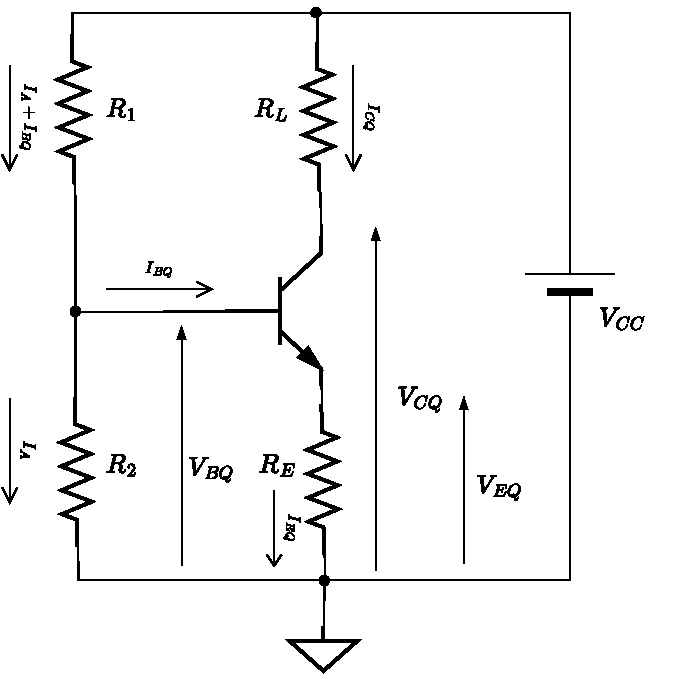
\includegraphics[width=0.45\linewidth]{img/43.pdf}
  \caption{電流帰還バイアス回路の原理図}
  \label{current_bias}
  \end{center}
\end{figure}


$I_{BQ} \approx 0$ と近似(他の電流と比べて小さいため)すると、$R_1$ を流れる電流は、全て$R_{2}$ に流れるので、\\
\begin{align}
  V_{BQ} \approx \frac{R_2}{R_1+R_2}V_{CC}
\end{align}
により、ベースのバイアス電圧が求まる。ベース電流がゼロなので、$r_b$ (ベース層の抵抗)による電圧降下はゼロである。
$I_{EQ} = \frac{V_{EQ}}{R_E}$ ($V_{EQ}$ は $R_E$ の両端電圧)\\
$V_{EQ} = V_{BQ} - V_{BE}$ ($V_{BE}$ は、前のシミュレーションで求めた約 0.7 V の値を使う。)\\
$I_{CQ} \approx I_{EQ} (I_{EQ} = I_{CQ} - I_{BQ} \approx 0)$\\
$V_{CQ} = V_{CC} - R_LI_{CQ}$\\
$I_{BQ} = \frac{I_{CQ}}{\beta_0}$ ($\beta_0$: 直流電流増幅率)

\mysubsection{回路の特徴}
\begin{enumerate}
  \setlength{\parskip}{0cm} % 段落間
  \setlength{\itemsep}{0cm} % 項目間
  \item 温度補償\\
  トランジスタの直流電流増幅率は、温度によって上昇する性質がある。
  $\beta_{0}$ 増加 → $I_{CQ}$ が増加 → $I_{EQ}$ も増加 → $R_{E}I_{EQ}$ が増加\\
  $V_{BE} = V_{BQ} - V_{CQ}$ より、$V_{BE}$ が減少 → $I_{BQ}$ が減少 → $I_{CQ}$ の増加を抑制する。
  \item 利点: 温度が変化した場合のバイアス安定度が高い。
  \item 欠点: $R_2$ を比較的小さく設定する関係で、これらの抵抗に流れる電流(ブリーダ電流)により、消費電流が大きくなる。
\end{enumerate}

\mysubsection{電流帰還バイアス回路の設計手順}
電流帰還バイアス回路を設計するためにあらかじめ条件が要求される。
\begin{enumerate}
  \setlength{\parskip}{0cm} % 段落間
  \setlength{\itemsep}{0cm} % 項目間
  \item 諸条件の設定
  \begin{itemize}
    \item 使用するトランジスタ:2SC1815
    \item 直流増幅率$\beta_0 = 213$
    \item $V_{BE} = 0.7386$ V
    \item $V_{CC} = 10$V
    \item バイアス点電流$I_{CO}=5.5$mA
    \item $I_{BO}= \frac{I_{CO}}{\beta_0} = \frac{5.5\times10^{-3}}{213} \approx 25.82 \mu$A
    \item $R_E$による電圧降下は、$V_{CC}$の10\verb|%| とする。
    \item $V_{CEO} = V_{RLO}$とする。
    \item ブリーダ電流$I_A$: $I_{BO}$ の20倍
  \end{itemize}
  \item $R_E$を求める\\
  $V_{EO} = R_EI_{EO} = 0.1V_{CC} = 1.0$ V $I_{EO} \approx I_{CO}$ より
  \begin{align}
    R_E = \frac{V_{EO}}{I_{CO}} = \frac{1}{5.5 \times 10^{-3}} \approx 181.818 \Omega    
  \end{align}

  \item $R_L$を求める\\
  $R_L$ に流れる電流 $I_{CO}$ について、$V_{CEO} = V_{CO} -V_{EO}$ と $R_LI_{CO}$ を等しくすると、出力信号の振幅を最大化できる。(動作点を負荷線の真ん中に選ぶ)
  \item ブリーダ電流$I_A$を求める。\\
  $20 \times I_{BO} = 20 \times 25.82 \mu$ A $= 0.5164$ mA
  \item $R_2$を求める\\
  $V_{BO} = R_2I_A$ より、
  \begin{align}
    R_2 = \frac{V_{BO}}{I_A} = \frac{(V_{EO}+V_{BE})}{I_A} = \frac{(1+0.7386)}{0.5164}\approx 3366.769946 \approx 3.4 \textrm{k}\Omega    
  \end{align}
  \item $R_1$を求める
  \begin{align}
    R_1 = \frac{(V_{CC} - (V_{EO}+V_{BE}))}{I_A+I_{BO}} = \frac{(10 - (1+0.7386))}{(0.5164 \times 10^{-3} + 25.82\mu)} = 15236.25097 \approx 15.2 \textrm{k}\Omega
  \end{align}
\end{enumerate}
% \mysection{エミッタ接地交流増幅回路の設計(原理・計算)}
図\ref{emit_kouryu}にエミッタ接地交流増幅回路を示す。ここでは、どのキャパシタが入力信号を遮断周波数に影響を与えるかを考える。
\begin{figure}[htbp]
  \begin{center}
  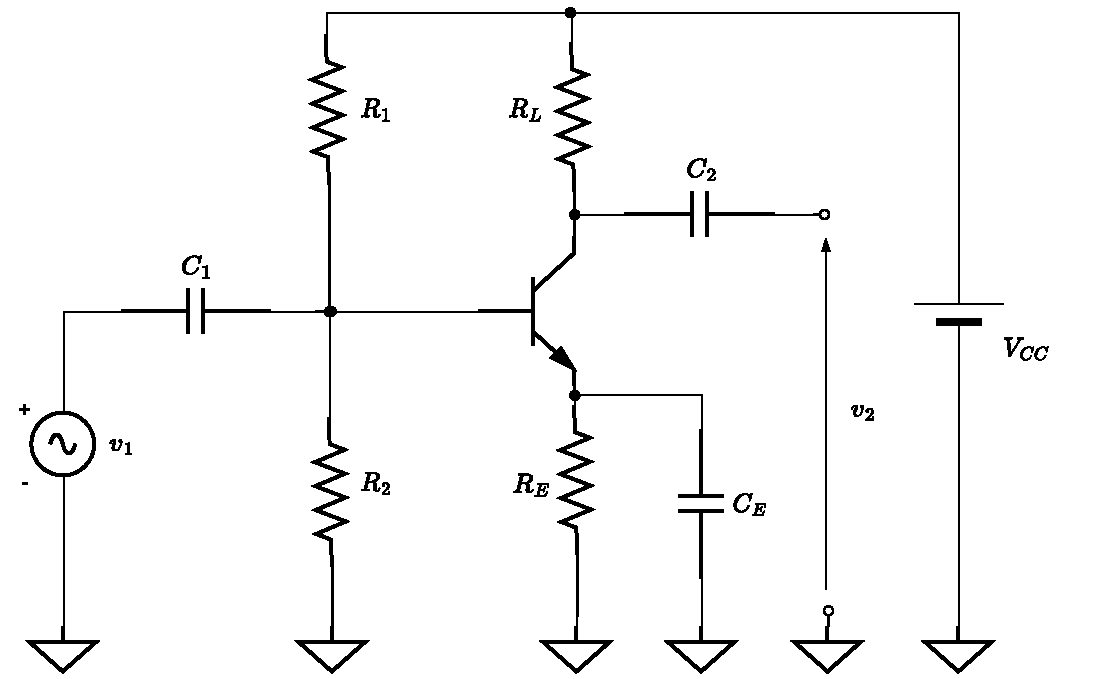
\includegraphics[width=0.68\linewidth]{img/45.pdf}
  \caption{エミッタ接地交流増幅回路}
  \label{emit_kouryu}
  \end{center}
\end{figure}

$C_{E}$: バイパスキャパシタ\\
$C_{1}, C_{2}$: 結合キャパシタ(直流信号を遮断して交流信号だけを通過)

\mysubsection{等価回路}
エミッタ接地微小信号等価回路と微小信号の変化分を表す特性を図に示す。
微小信号とは、小さな振幅の交流信号のことである。
$r_e$ は、ベース - エミッタ間の pn 接合ダイオードを抵抗に置き換えたものである。
直流に対しては、この pn 接合はダイオードと考えられるが、ベースの入力信号が微小変化する場合には、$V_{BE}$ の変化に対してエミッタ電流 $I_E$ の変化が比例して変化するものと考えられる。
\begin{figure}[htb]
  \begin{center}
  \subfigure[エミッタ接地微小信号等価回路]{
  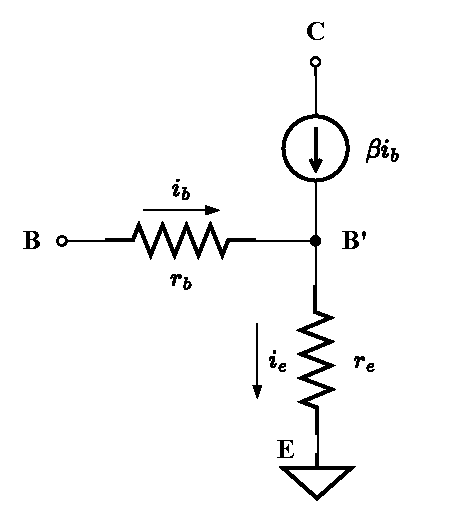
\includegraphics[width=.45\columnwidth]{img/46.pdf}
  }
  \subfigure[微小信号の変化分を表す特性($V_{BE}$-$I_E$特性の再喝)]{
  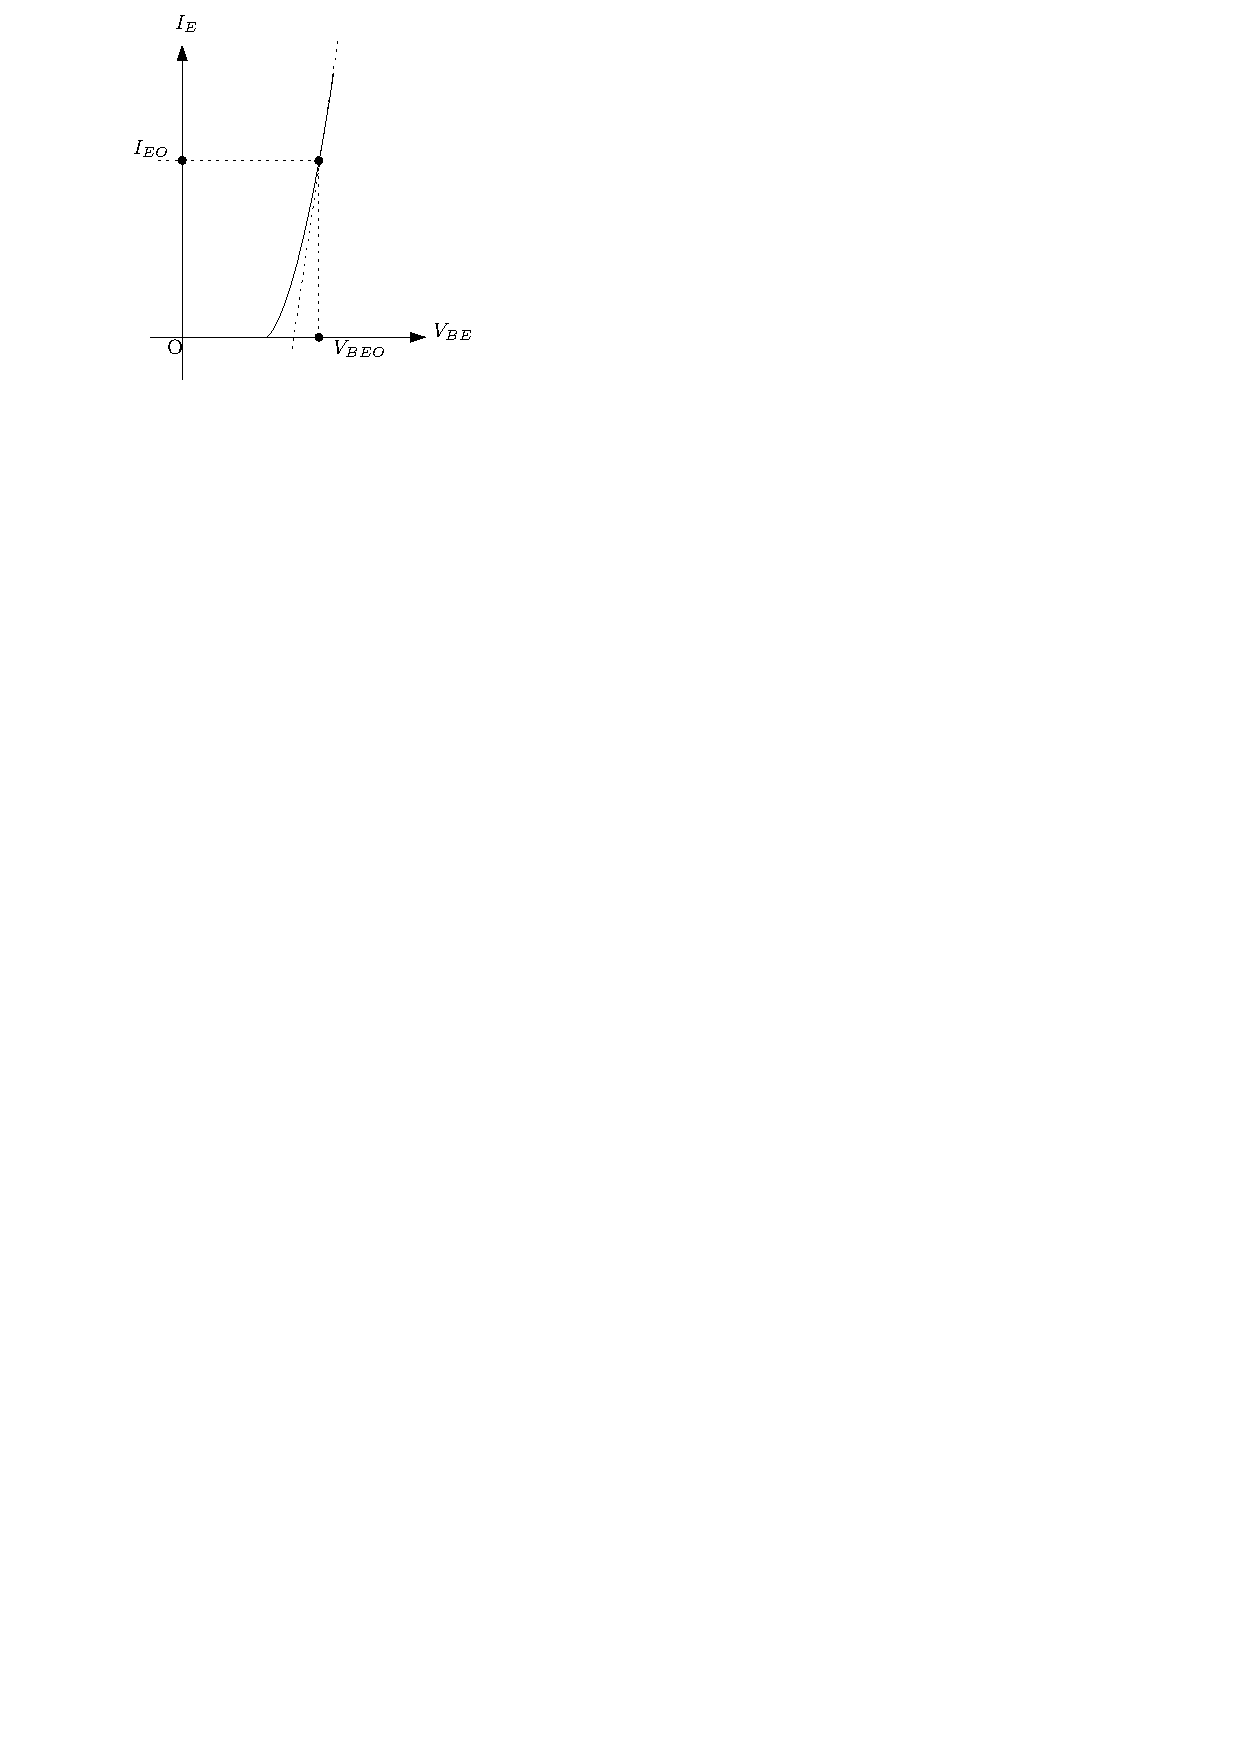
\includegraphics[width=.45\columnwidth]{img/47.pdf}
  }
  \caption{微小信号等価回路の原理}
  \label{vbe_ie}
  \end{center}
\end{figure}

$I_E \approx I_S \exp(\frac{q}{kT}V_{BE})$ を $V_{BE}$ で微分すると(これが、$I_E$-$V_{BE}$曲線の傾きとなる。)\\
\begin{align}
  & \frac{1}{r_e} = \frac{dI_E}{dV_{BE}} \approx \frac{q}{kT}I_S\exp(\frac{q}{kT}V_{BE}) = \frac{q}{kT}I_E\\
  & r_e = \frac{kT}{q}\cdot\frac{1}{I_{EO}} \approx \frac{0.026}{I_{EO}}
\end{align}

\mysubsection{電圧増幅度の計算}
図\ref{emit_touka}に、微小信号等価回路を利用して描いたエミッタ接地交流等価回路を示す。

\begin{figure}[htbp]
  \begin{center}
  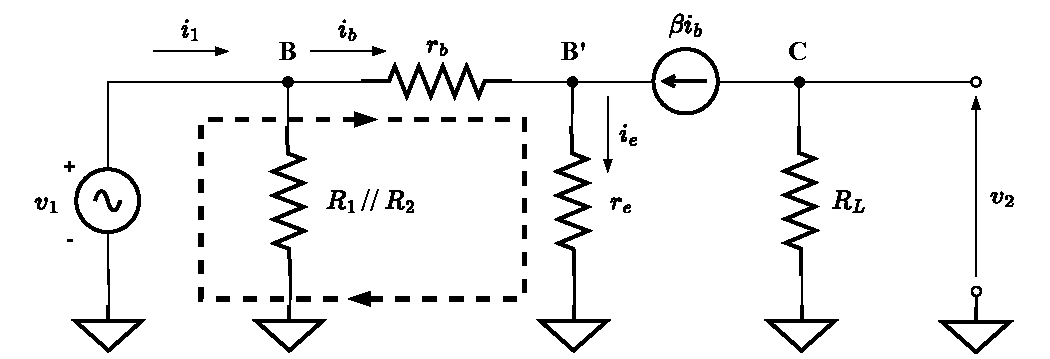
\includegraphics[width=0.8\linewidth]{img/48.pdf}
  \caption{エミッタ接地交流増幅回路の等価回路}
  \label{emit_touka}
  \end{center}
\end{figure}

\begin{description}
  \item [入力インピーダンス]: $R_1//R_2$と$Z_i$が並列に接続されている。\\
  ($Z_i$は、ベース端子から見た入力インピーダンス)
  ここで、$Z_i = v_1/i_b$より、点線のループに沿ってキルヒホッフの法則を適用すると、
  \begin{align}
    v_1 = r_bi_b+r_ei_e \label{eq1}
  \end{align}
  B'点にキルヒホッフの電流則を適用すると、
  \begin{align}
    i_e = (1+\beta)i_b \label{eq2}
  \end{align}
  式\eqref{eq1}、\eqref{eq2}より、$i_e$ を消去して、
  \begin{align}
    v_1 = r_bi_b+r_e(1+\beta)i_b
  \end{align}
よってベースから見た入力インピーダンス $Z_i$ は、
  \begin{align}
    Z_i = \frac{v_1}{i_b} = r_b+(1+\beta)r_e
  \end{align}
$Z_i$ を用いると、エミッタ接地回路の入力端子から見たインピーダンス $Z_{in}$ は、
  \begin{align}
    Z_{in} = R_1//R_2//Z_i
  \end{align}
となる。
  \item [電圧増幅度]: 負荷抵抗 $R_L$ には下から上に流れる電流 $\beta i_b$ が流れている。\\
  よって、出力電圧 $v_2$ は、逆の極性を持つため、
  \begin{align}
    & v_2 = - R_L\beta i_b\\
    & i_b = \frac{v_1}{r_b+(1+\beta)r_e}\\
    & A_v = \frac{v_2}{v_1} = \frac{-\beta R_L}{r_b+(1+\beta)r_e} = \frac{-\beta R_L}{Z_i}    
  \end{align}

\end{description}

\mysubsection{$C_1$ による遮断周波数 $f_{C1}$}
  入力側の結合キャパシタ $C_1$を考慮した入力部の等価回路を図\ref{C1}に示す。

  \begin{figure}[htbp]
    \begin{center}
    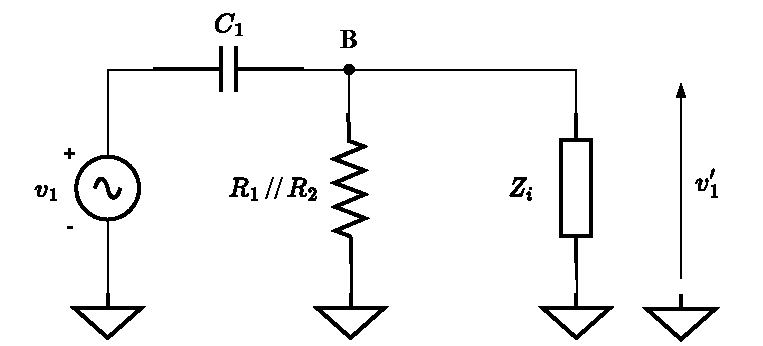
\includegraphics[width=0.8\linewidth]{img/49.pdf}
    \caption{$C_1$を考慮したエミッタ接地交流増幅回路の等価回路}
    \label{C1}
    \end{center}
  \end{figure}
  $v_1'$: ベースへの交流入力電圧 $v_1$: 元の入力信号として、\\
  電圧 $v_1$$v_1'$との比を求めると、
  \begin{align}
    & \frac{v_1'}{v_1} = \frac{R_1//R_2//Z_i}{\frac{1}{j\omega C_1}+R_1//R_2//Z_i} = \frac{1}{1+\frac{1}{j\omega C_1(R_1//R_2//Z_i)}}\\
    & Z_i = \frac{v_1}{i_b} = r_b+(1+\beta)r_e    
  \end{align}

  キャパシタ $C_1$ を入れた時の電圧増幅度 $A'_v = \frac{v_2}{v_1}$ は、$A_v = \frac{v_2}{v'_1}$ として、
  \begin{align}
    A'_v = \frac{v_2}{v_1} = \frac{v'_1}{v_1}\cdot\frac{v_2}{v'_1} = A_v\frac{v'_1}{v_1} = \frac{-\beta R_L}{Z_i} \cdot \frac{1}{1+\frac{1}{j\omega C_1(R_1//R_2//Z_i)}}    
  \end{align}

  $A'_v$ の絶対値、(振幅伝達関数)は、
  \begin{align}
    |A'_v| = \frac{\beta R_L}{Z_i} \times \frac{1}{\sqrt{1+(\frac{1}{\omega C_1(R_1//R_2//Z_i})^2}}
  \end{align}
  となる。
  $\frac{\beta R_L}{Z_i}$は、全てのキャパシタを短絡して考えた $A_v$ の式と同じである。
  この増幅度から、$\frac{1}{\sqrt{2}}$ に低下する周波数(低域遮断周波数$f_{C1}$)は、
  $\omega C_1(R_1//R_2//Z_i) = 1$より、
  \begin{align}
    & 2\pi f_{C1}C_1(R_1 // R_2 // Z_i) = 1\\
    & C_1 = \frac{1}{2\pi f_{C1} (R_1//R_2//Z_i)} = 1    
  \end{align}


\mysubsection{$C_2$による遮断周波数$f_{C2}$}
入力側の結合キャパシタ$C_2$を入れた入力部の等価回路を図\ref{c2}に示す。
\begin{figure}[htbp]
  \begin{center}
  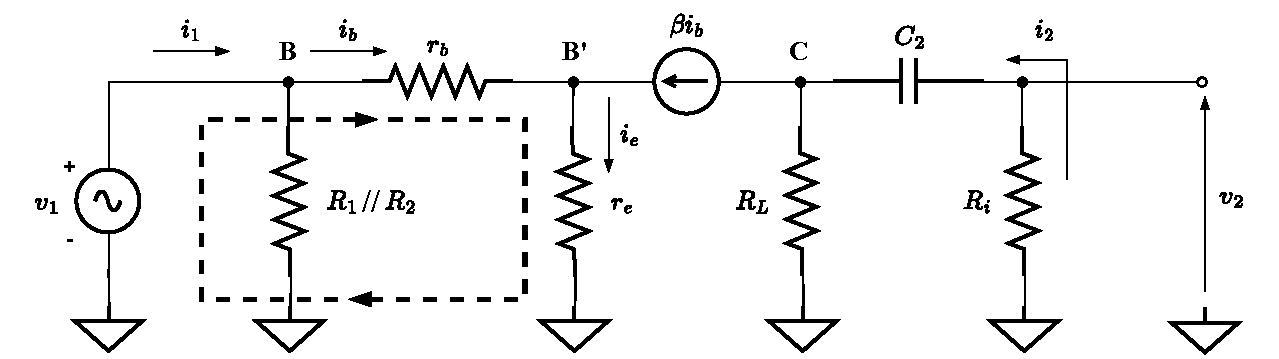
\includegraphics[width=0.8\linewidth]{img/50.pdf}
  \caption{$C_2$を考慮したエミッタ接地交流増幅回路の等価回路}
  \label{c2}
  \end{center}
\end{figure}
図の点線に沿ってキルヒホッフの電圧則を適用すると、
\begin{align}
  v_1 = r_bi_b+(1+\beta)r_ei_b  
\end{align}

出力側に流れる電流$i_2$を電流源$\beta i_b$から求めると、出力側の回路は$R_L$と、直列の$C_2-R_i$が並列接続された形であるため、\\
\begin{align}
  i_2 = \beta i_b \times \frac{R_L}{R_L+(\frac{1}{j\omega C_2}+R_i)}
\end{align}
で求まる。また、出力側電圧$v_2$は、
\begin{align}
  v_2 = - i_2R_i
\end{align}
よって、電圧増幅度$A_v$は、
\begin{align}
\begin{aligned}
  A_v & = \frac{v_2}{v_1} = \frac{-i_2R_i}{r_bi_b+(1+\beta)r_ei_b} = \frac{\frac{-\beta R_LR_i}{R_L+(\frac{1}{j\omega C_2}+R_i)}}{r_b+(1+\beta)r_e}\\
  & = \frac{-\beta}{r_bi_b+(1+\beta)r_ei_b} \cdot \frac{R_LR_i}{R_L+(\frac{1}{j\omega C_2}+R_i)} = \frac{-\beta}{r_bi_b+(1+\beta)r_ei_b} \cdot \frac{\frac{R_LR_i}{R_L+R_i}}{1+\frac{1}{j\omega C_2(R_L+R_i)}}\\
  & = \frac{-\beta R'_L}{r_bi_b+(1+\beta)r_ei_b} \cdot \frac{1}{1+\frac{1}{j\omega C_2(R_L+R_i)}}
\end{aligned}
\end{align}
と求まる。($R'_L = R_L//R_i$)\\
$\frac{-\beta R'_L}{Z_i} \cdot \frac{1}{1+\frac{1}{j\omega C_2(R_L+R_i)}}$ と、$-\frac{\beta R_L}{Z_i}$ と見比べると、$C_2$ を短絡して考えられる 周蓮での増幅度に相当する。つまり、$R_L$ と次段の入力インピーダンス $R_i$ が並列接続された形で増幅度が決まる。
\begin{align}
  |A_v| = \frac{\beta R'_L}{Z_i} \cdot \frac{1}{\sqrt{1+(\frac{1}{(\omega C_2(R_L+R_i)})^2}}  
\end{align}

$C_2$ を短絡して考えた場合の値 $\frac{\beta R'_L}{Z_i}$ に対して、増幅度が $1/sqrt{2}$ となる周波数(低域遮断周波数 $f_{C2}$)は、$\omega C_2(R_L+R_i) = 1$、$2\pi f_{C2} C_2(R_L+R_i) = 1$ より、
\begin{align}
  f_{C2} = \frac{1}{2\pi C_2(R_L+R_i)}  
\end{align}

\mysubsection{$C_E$による遮断周波数 $f_{CE}$}
抵抗 $R_E$ に並列にバイパスキャパシタ$C_E$を入れた等価回路を図\ref{ce}に示す。
\begin{figure}[htbp]
  \begin{center}
  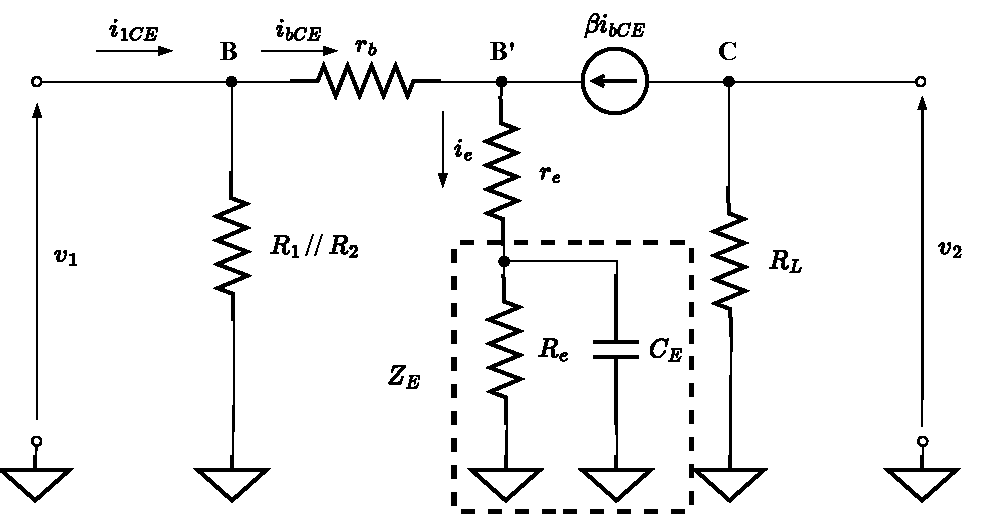
\includegraphics[width=0.8\linewidth]{img/51.pdf}
  \caption{$C_E$を考慮したエミッタ接地交流増幅回路の等価回路}
  \label{ce}
  \end{center}
\end{figure}

$C_E, R_E$ の並列インピーダンス $Z_E$は、
\begin{align}
  Z_E = \frac{R_E \cdot \frac{1}{j\omega C_E}}{R_E+\frac{1}{j\omega C_E}} = \frac{R_E}{1+j\omega C_ER_E} \label{ze}
\end{align}

$C_E$ が短絡している場合、$Z_E = 0$ となる。$v_1 \rightarrow r_b \rightarrow r_e$のループにキルヒホッフの電圧則を適用した式 $v_1 = r_bi_{bCE}+r_e(1+\beta)i_{bCE}$ を用いて、
\begin{align}
  Z_i = \frac{v_1}{i_{bCE}} = r_b+(1+\beta)r_e
\end{align}
となる。($Z_i$ベース端子B から見たトランジスタの入力インピーダンス)

$r_b: 50 ~ 500 \Omega$ 程度 $\beta$: 100 ~ 500 程度 ダイオードの交流等価回路 $r_e$: 数10 $\Omega$ $(1+\beta)r_e >> r_b, \beta >> 1$ として、
\begin{align}
  Z_i \approx (1+\beta)r_e \approx \beta r_e \label{zi}
\end{align}
となる。

電圧増幅度 $A_v = \frac{v_2}{v_1}$ について、$v_1 \rightarrow r_b \rightarrow r_e \rightarrow Z_E$ のループにキルヒホッフの電圧則を適用すると

$v_1 = r_b i_{bCE}+(r_e+Z_E)(1+\beta)i_{bCE}$
$= [r_b+(1+\beta)(r_e+Z_E)]i_{bCE} = [r_b+(1+\beta)r_e+(1+\beta)Z_E]i_{bCE}$
$= [Z_i+(1+\beta)Z_E]i_{bCE}$ となる。
$v_2 = -R_L\beta i_{bCE}$ ($v_2$ は、電流$\beta i_{bCE}$ が負荷抵抗 $R_L$ を下から上に流れる。)

\begin{align}
  A_v = \frac{v_2}{v_1} =\frac{-\beta R_L}{Z_i+(1+\beta)Z_E} \label{av}  
\end{align}

式\eqref{av}を図\eqref{ze}、図\eqref{zi}に代入して、
\begin{align}
  \begin{aligned}
  A_v & = \frac{-\beta R_L}{Z_i+(1+\beta)Z_E} \approx \frac{-\beta R_L}{Z_i+\beta \frac{R_E}{1+j\omega C_E R_E}}\\
  & = \frac{-\beta R_L(1+j\omega C_E R_E)}{Z_i(1+j\omega C_ER_E)+\beta R_E} = -\beta R_L \cdot \frac{1+j\omega C_E R_E}{Z_i+\beta R_E+j\omega C_ER_EZ_i} \approx -\beta R_L \cdot \frac{1+j\omega C_E R_E}{\beta r_e+\beta R_E + j\omega C_E R_E Z_i}\\
  & = -\beta R_L R_E \cdot \frac{1+j\omega C_ER_E}{\beta(r_e+R_E)+j\omega C_E R_E Z_i} \approx -\beta R_L \cdot \frac{1+j\omega C_E R_E}{\beta R_E + j\omega C_E R_E Z_i}\\
  & = -\frac{\beta R_L}{R_E} \cdot \frac{1+j\omega C_E R_E}{\beta + j\omega C_E Z_i} = -\frac{R_L}{R_E} \cdot \frac{1+j\omega C_E R_E}{1+j\omega C_E Z_i/\beta} \\ \label{}
  \end{aligned}
\end{align}
式\eqref{zi}より、
\begin{align}
  A_v \approx -\frac{R_L}{R_E}\cdot\frac{1+j\omega C_ER_E}{1+j\omega C_EZ_i/\beta} \approx -\frac{R_L}{R_E}\cdot \frac{1+j\omega C_E R_E}{1+j\omega C_E r_e}
\end{align}
$f \to \infty, \omega \to \infty$ の場合、\\
$\left.A_v\right|_{\omega \to 0} \approx -\frac{R_L}{R_E}$ と一定値(低域の電圧増幅度) になり、\\
$\left.A_v\right|_{\omega \to \infty} \approx -\frac{R_L}{r_e} \leftarrow$ ロピタルの定理\\
と、一定値(中域での電圧増幅度)となる。

$-\frac{R_L}{R_E} \cdot \frac{1+j\omega C_E R_E}{1+j\omega C_E r_e}$ の分母分子に関係する特徴的な周波数について

\begin{align}
  f_{CE1} = \frac{1}{2\pi C_E Z_i/\beta} \approx \frac{1}{2\pi C_E r_e}\\
  f_{CE2} = \frac{1}{2\pi C_E R_E}\\
  A_v \approx -\frac{R_L}{R_E} \cdot \frac{1+j(f/f_{CE2})}{1+j(f/f_{CE1})}\\
  A_v \approx -\frac{R_L}{R_E} \cdot \frac{1+j(f/f_{CE2})}{1+j(f/f_{CE1})}\\
  |A_v| \approx \frac{R_L}{R_E} \cdot \sqrt{\frac{1+(f/f_{CE2})^2}{1+(f/f_{CE1})^2}}
\end{align}

この式は、低周波数側から周波数を増加させるとき、$f_{CE2}, f_{CE1}$ で2回折れ曲がる形の関数である。

$f_{CE2}$ は、$C_E R_E$ で決まる周波数
低周波数 → 高周波数に増加するときに増幅度が上りはじめる周波数

$f_{CE1}$ は、時定数 $C_E r_e$ で決まる周波数で、高周波 → 低周波数に減少するときに
増幅度が下がりはじめる周波数である。したがって、バイパスキャパシタ $C_E$ を含む図の等価回路では、低域遮断周波数は、$f_{CE1}$ となる。

\mysubsection{低域遮断周波数のまとめ}
入力側キャパシタ $C_1$: $f_{C1} = \frac{1}{2\pi C_1(R_1//R_2//Z_i)}$\\
出力側キャパシタ $C_2$: $f_{C2} = \frac{1}{2\pi C_2(R_L+R_i)}$\\
バイパスキャパシタ $C_E$: $f_{CE1} = \frac{1}{2\pi C_E Z_i/\beta} \approx \frac{1}{2\pi C_E r_e}$\\

$R_1, R_2, R_L, R_i, Z_i$ が、k$\Omega$ オーダに対し、$r_e \approx \frac{Z_i}{\beta}$ は、\\
1 ~ 10 $\Omega$ オーダ各キャパシタの静電容量を同じにすると、$C_E$ による周波数 $f_{CE1}$ が最も大きな値となる。つまり、低域遮断周波数は、トランジスタの交流増幅率の低下、ベース- コレクタ間容量によるベース端子への逆位相信号入力(負帰還)、回路を組み立てる配線の分布容量など複数の要因がからみ合っており、高域遮断周波数の設計には、より高度な回路に関する知見が必要である。

\mysubsection{諸量計算$r_e$、$A_v$、低域遮断周波数}
$r_e, A_v(電圧増幅度), 低域遮断周波数 f_{CE1}, f_{C1}, f_{C2}$\\
条件1 $C_1, C_2$は、$100 \mu$F を使う
\begin{enumerate}
  \setlength{\parskip}{0cm} % 段落間
  \setlength{\itemsep}{0cm} % 項目間
  \item $r_e \approx \frac{kT}{q} \cdot \frac{1}{I_{EQ}}$
  $r_e \approx \frac{0.026}{I_{EO}} (I_{EO} \approx I_{CO}) (\frac{kT}{q} は定数)$
  \item $A_v = \frac{v_2}{v_1} = -\frac{\beta R_L}{Z_i} = -\frac{R_L}{Z_i/\beta} \approx -\frac{R_L}{r_e} = \frac{506}{3.3} \approx -153$
\end{enumerate}

条件2: 低域遮断周波数$f_{CE1} = 20$ Hz として設計)
$$f_{CE1} \approx \frac{1}{2\pi C_E r_e} \Rightarrow C_E \approx \frac{1}{2\pi f_{CE1}r_e}$$


\mysection{エミッタ接地交流増幅回路の設計手順}
\begin{enumerate}
  \setlength{\parskip}{0cm}
  \setlength{\itemsep}{0cm}
  \item $r_e \approx \frac{0.026}{I_{EO}} \approx \frac{0.026}{I_{CO}} = \frac{26\times10^{-3}}{5.5 \times 10^{-3}} \approx 4.7272 [\Omega]$
  \item $A_v = \frac{v_2}{v_1} = -\frac{\beta R_L}{Z_i} = -\frac{R_L}{Z_i/\beta} \approx -\frac{818.18}{4.72} = -173.3432...$
  \item $C_E$: 低域遮断周波数を 20 Hz として設定(可聴周波数の下限)
  \begin{align}
    f_{CE1} \approx \frac{1}{2\pi C_Er_e} \Rightarrow C_E \approx \frac{1}{2\pi f_{CE1} r_e} \approx \frac{1}{2\pi \times 20 \times 4.72} = 1.68596 \times 10^{-3} = 1686 \mu\textrm{F}
  \end{align}
\end{enumerate}
$C_1, C_2は、100 \mu\textrm{F} より、次段の入力インピーダンスを R_i = 1\textrm{k}\Omega と仮定$

\begin{align}
  & f_{C1} = \frac{1}{2\pi C_1(R_1//R_2//Z_i)} \approx \frac{10^4}{2\pi \times (15.2\times10^3//3.4\times10^3//10^3)} \approx \frac{10^4}{2\pi \times 735.344} \approx 2.1643\textrm{Hz}\\
  & f_{C2} = \frac{1}{2\pi C_2(R_L+R_i)} \approx \frac{1}{2\pi \times 10^{-4} \times 1.818 \times 10^3} = 0.8754[\textrm{Hz}]  
\end{align}

$f_{C1}, f_{C2}$は、20 Hz と比べてかなり小さい。
\end{document}